\subsection*{2. Schritt: Singulärwert-Zerlegung}

Wir führen zunächst eine Singulärwert-Zerlegung von $A_0$ durch.

\begin{align*}
    \tilde V \Sigma \tilde W^\ast = A_0 \in \C^{N \times j},
    \quad
    \tilde V \in \U_N(\C),
    \quad
    \tilde W \in \U_j(\C),
    \quad
    \Sigma_{l, k} = \sigma_l \delta_{l, k},
    \quad
    l = 1, \dots, N,
    \quad
    k = 1, \dots, j
\end{align*}

\begin{remark}

    Sei $f \in \Lin(V, W)$ vom Vektorraum $V$ in den Vektorraum $W$, $B \subset V$ eine Basis, und $A$ eine Matrix-Darstellung von $f$.
    Dann gelten folgende Äquivalenzen.

    \begin{multline*}
        \text{$A$ hat vollen Spaltenrang}
        \iff
        \text{$A$ hat linear unabhängige Spalten} \\
        \iff
        \text{$f$ ist injektiv}
        \iff
        \text{$f(B) \subset W$ ist linear unabhängig}
    \end{multline*}

    \begin{multline*}
        \text{$A$ hat vollen Zeilenrang}
        \iff
        \text{$A$ hat linear unabhängige Zeilen} \\
        \iff
        \text{$f$ ist surjektiv}
        \iff
        \text{$f(B) \subset W$ ist Erzeugendensystem}
    \end{multline*}

\end{remark}


Nun haben wir angenommen, dass $V, W \in \C^{N \times J}$ vollen Spaltenrang $J$ haben und $\hat V$ vollen Spaltenrang $j$.
$W^\ast$ hat also vollen Zeilenrang $J$.
Abbildung \ref{fig:rang_1} illustriert, dass $A_0 = V W^\ast \hat V$ genau $J$ linear unabhängige Spalten hat, also Spaltenrang $J$.

\begin{figure}[!ht]
    \centering
    \begin{tikzpicture}[scale = 0.5]

        \draw (0,  0) rectangle (2,  6);
        \draw (6,  0) rectangle (8,  6);
        \draw (12, 0) rectangle (14, 6);
        \draw (18, 0) rectangle (20, 6);

        \draw (0, 1) -- (2, 1);
        \draw (0, 5) -- (2, 5);

        \draw [dotted] (2, 1) -- (6, 0);
        \draw [dotted] (2, 5) -- (6, 6);

        \draw [dotted] (8, 0) -- (12, 2);
        \draw [dotted] (8, 6) -- (12, 4);

        \draw (12, 2) -- (14, 2);
        \draw (12, 4) -- (14, 4);

        \draw [dotted] (14, 2) -- (18, 0);
        \draw [dotted] (14, 4) -- (18, 6);

        \draw (1,  3) node {$\C^j$};
        \draw (4,  3) node {$\xrightarrow[\text{injektiv}]{\hat V}$};
        \draw (7,  3) node {$\C^N$};
        \draw (10, 3) node {$\xrightarrow[\text{surjektiv}]{W^\ast}$};
        \draw (13, 3) node {$\C^J$};
        \draw (16, 3) node {$\xrightarrow[\text{injektiv}]{V}$};
        \draw (19, 3) node {$\C^N$};

    \end{tikzpicture}
    \caption{}
    \label{fig:rang_1}
\end{figure}

Matrizen haben genau dann denselben Rang, wenn sie äquivalent sind.

\begin{align*}
    \begin{pmatrix}
        \diag(\sigma_1, \dots, \sigma_J, \dots, \sigma_j) \\
        0_{(N - j) \times j}
    \end{pmatrix}
    =
    \Sigma
    \equiv
    \tilde V \Sigma \tilde W^\ast
    =
    A_0
    \equiv
    \begin{pmatrix}
        I_J \enspace 0_{J \times (j - J)} \\ 0_{(N - J) \times j}
    \end{pmatrix}
\end{align*}

Damit verschwinden die letzten Singulärwerte $\sigma_{J+1} = \cdots = \sigma_j = 0$.
Somit können wir statt der vollen Singulärwert-Zerlegung (indiziert mit \Quote{full}) eine reduzierte (indiziert mit \Quote{reduced}) verwenden.

\begin{align*}
    A_0
    =
    \tilde V_\mathrm{full} \Sigma_\mathrm{full} \tilde W_\mathrm{full}^\ast
    =
    \begin{pmatrix}
        \tilde V_\mathrm{reduced} & \ast
    \end{pmatrix}
    \begin{pmatrix}
        \Sigma_\mathrm{reduced} & 0_{J \times (j - J)}       \\
        0_{(N - J) \times J}    & 0_{(N - J) \times (j - J)}
    \end{pmatrix}
    \begin{pmatrix}
        \tilde W_\mathrm{reduced}^\ast \\ \ast
    \end{pmatrix}
    =
    \tilde V_\mathrm{reduced} \Sigma_\mathrm{reduced} \tilde W_\mathrm{reduced}^\ast
\end{align*}

Die $\tilde V_\mathrm{full}$ und $\tilde W_\mathrm{full}$ sind ja unitär, d.h. ihre Adjungierten waren ihre Inversen.

\begin{align*}
    \implies
    I_{N \times N}
    =
    \tilde V_\mathrm{full}^\ast \tilde V_\mathrm{full}
    =
    \begin{pmatrix}
        \tilde V_\mathrm{reduced}^\ast \\ \ast
    \end{pmatrix}
    \begin{pmatrix}
        \tilde V_\mathrm{reduced} & \ast
    \end{pmatrix}
    =
    \begin{pmatrix}
        \tilde V_\mathrm{reduced}^\ast \tilde V_\mathrm{reduced} & \ast \\
        \ast                                                     & \ast
    \end{pmatrix}
\end{align*}

Eine analoge Rechnung kann man, mit $j$ anstelle von $N$, für $\tilde W_\mathrm{reduced}$ machen.
Insgesamt erhalten wir also folgende Tatsachen über unsere reduzierte Singulärwert-Zerlegung.
Wir vereinbaren, ab sofort nur noch die reduzierte Singulärwert-Zerlegung zu verwenden und den Index wegzulassen.

\begin{align} \label{eq:singulärwert_zerlegung}
    \tilde V^\ast \tilde V
    =
    \tilde W^\ast \tilde W
    =
    I_{J \times J},
    \quad
    \Sigma = \diag(\sigma_1, \dots, \sigma_J),
    \quad
    A_0 = \tilde V \Sigma \tilde W^\ast
\end{align}

$\tilde V$ hat, als Teil-Matrix einer unitären, vollen Spaltenrang $J$ hat.
$\tilde V^\ast$ hat also vollen Zeilenrang $J$.
Abbildung \ref{fig:rang_2} illustriert, dass $S := \tilde V^\ast V \in \C^{J \times J}$ genau $J$ linear unabhängige Spalten hat, also $S \in \GL_J(\C)$.

\begin{figure}[!ht]
    \centering
    \begin{tikzpicture}[scale = 0.5]

        \draw (0,  0) rectangle (2,  6);
        \draw (6,  0) rectangle (8,  6);
        \draw (12, 0) rectangle (14, 6);

        \draw (0, 2) -- (2, 2);
        \draw (0, 4) -- (2, 4);

        \draw [dotted] (2, 2) -- (6, 0);
        \draw [dotted] (2, 4) -- (6, 6);

        \draw [dotted] (8, 0) -- (12, 2);
        \draw [dotted] (8, 6) -- (12, 4);

        \draw (12, 2) -- (14, 2);
        \draw (12, 4) -- (14, 4);

        \draw (1,  3) node {$\C^J$};
        \draw (4,  3) node {$\xrightarrow[\text{injektiv}]{V}$};
        \draw (7,  3) node {$\C^N$};
        \draw (10, 3) node {$\xrightarrow[\text{surjektiv}]{\tilde V^\ast}$};
        \draw (13, 3) node {$\C^J$};

    \end{tikzpicture}
    \caption{}
    \label{fig:rang_2}
\end{figure}

In den folgenden Gleichungsketten wird bei \Quote{!} die jeweils vorgerige eingesetzt.

\begin{align*}
    & \implies
    \Sigma \tilde W^\ast
    \stackrel
    {
        \eqref{eq:singulärwert_zerlegung}
    }{=}
    \tilde V^\ast \tilde V \Sigma \tilde W^\ast
    \stackrel
    {
        \eqref{eq:singulärwert_zerlegung}
    }{=}
    \tilde V^\ast A_0
    \stackrel
    {
        \eqref{eq:integral_matrizen_resultat}
    }{=}
    \tilde V^\ast V W^\ast \hat V
    =
    S W^\ast \hat V \\
    & \implies
    A_1
    \stackrel
    {
        \eqref{eq:integral_matrizen_resultat}
    }{=}
    V D W^\ast \hat V
    \stackrel{!}{=}
    V D S^{-1} \Sigma \tilde W^\ast \\
    & \implies
    \tilde V^\ast A_1 \tilde W \Sigma^{-1}
    \stackrel{!}{=}
    \tilde V^\ast V D S^{-1} \Sigma \tilde W^\ast \tilde W \Sigma^{-1}
    =
    S D S^{-1}
    \approx
    D
\end{align*}

Somit ist die Diagonalmatrix $D$, welche ja die gesuchten Eigenwerte enthält, ähnlich zur Matrix $\tilde V^\ast A_1 \tilde W \Sigma^{-1}$.
Ähnliche Matrizen haben dieselben Eigenwerte.
